\section{Introduction}
\label{pk:sec:intro}

Statistical models of game outcomes have a rich and diverse history, beginning with Zermelo almost a century ago (c.f. Section~\ref{in:sec:btmodel}).
In this chapter, we revisit his ideas and highlight their connections to modern machine-learning techniques.
In particular, we show how the Bradley--Terry model can be cast as a Gaussian-process classification model.
The Gaussian-process framework provides two key advantages.
First, it brings all the benefits of Bayesian inference.
In particular it provides a principled way to deal with the uncertainty associated with noisy observations and with predictions.
Second, it opens up new modeling perspectives through the specification of kernel functions.

Equipped with this, we study the problem of predicting outcomes of football matches between national teams.
We identify two key challenges,
\begin{enuminline}
\item that of \emph{data sparsity} (national teams usually play no more than ten matches per year), and
\item that of \emph{data staleness} (the team roster is constantly evolving).
\end{enuminline}
Taking inspiration from the observation that national teams' players frequently face each other in competitions between clubs (see Figure~\ref{pk:fig:sankey}), we show that these two difficulties can be addressed by the introduction of a \emph{player kernel}.
This kernel relates any two matches through the players lined up on the field, and makes it possible to seamlessly use matches between clubs to improve a predictive model ultimately used for matches between national teams.
This is beneficial because, in contrast to national teams, clubs play much more frequently, hence more data are available to train the model.
This also implicitly addresses the staleness problem, as a team is defined by the set of players present at a given match.

\begin{figure}
  \centering
  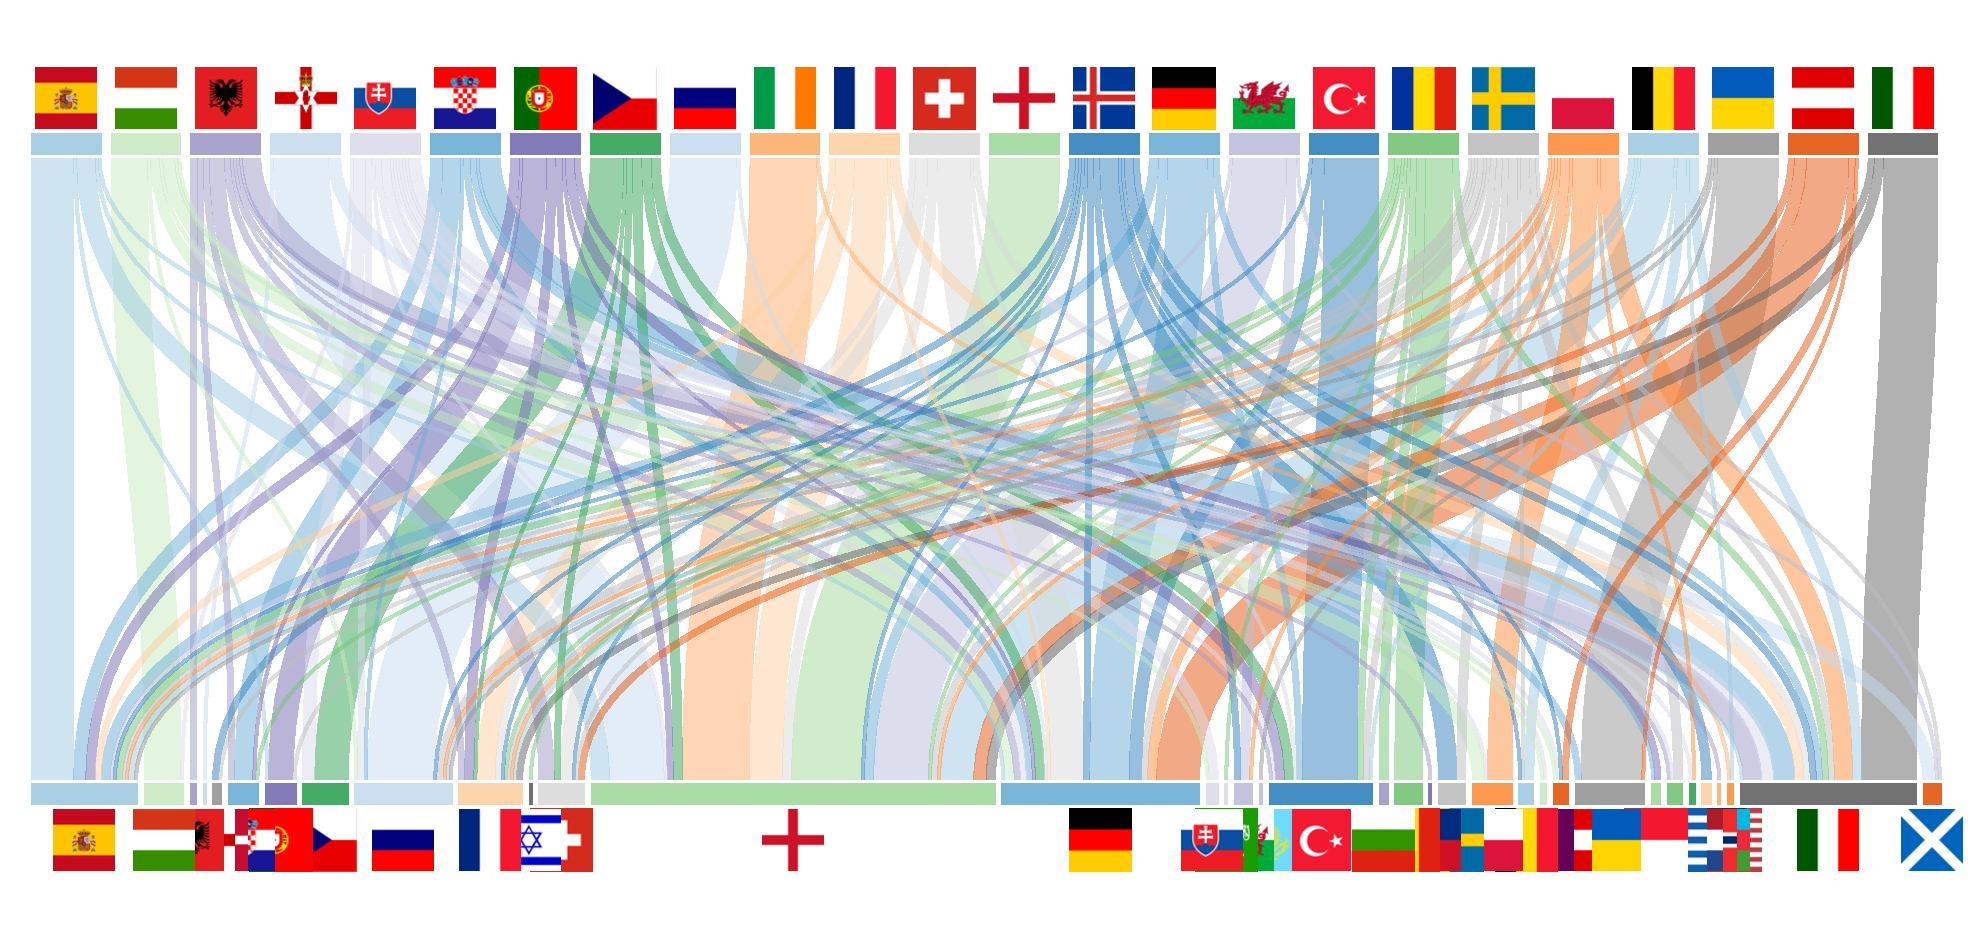
\includegraphics[width=\linewidth]{pk-sankey}
  \caption{
  Players of national teams qualified for the Euro 2016 (top row) are playing in clubs across Europe and beyond (bottom row).
  The English, German and Italian club championships contain the most selected players.
}
  \label{pk:fig:sankey}
\end{figure}

\paragraph{Outline of the Chapter}
The remainder of this short chapter is organized as follows.
We review related work in Section~\ref{pk:sec:relwork}.
In Section~\ref{pk:sec:methods}, we formalize the link between the Bradley--Terry model and Gaussian-process classification, and present the player kernel.
Then, in Section~\ref{pk:sec:evaluation}, we evaluate our predictive model on the Euro 2008, 2012 and 2016 final tournaments.
